\section{exercise e}

In this exercise we where going to compare our code with a manufactured solution

\begin{equation}
 u(x,t) = t \int_0^x q(1-q) dq = tx^2\left( \frac{1}{2} - \frac{x}{3}\right)
 \label{eq:manufactured}
\end{equation}

The way we do this is to find some $f(x,t)$ that satisfy the manufactured solution. This $f(x,t)$ is given as

\begin{equation}
 -\rho x^3 + \frac{\rho x^2}{2} + \frac{8 t^3 x^7}{9} - \frac{28 t^3 x^6}{9} + \frac{7 t^3 x^5}{2} - \frac{5 t^3 x^4}{4} +2 tx - t   
\end{equation}

In our python program we just use the Expression function

\begin{lstlisting}
f = Expression('-rho*pow(x[0],3)/3.0 + rho*pow(x[0],2)/2.0\
			   + pow(t,3)*(8.0*pow(x[0],7)/9.0 - 28.0*pow(x[0],6)/9.0 + 7.0*pow(x[0],5)/2.0 - 5.0*pow(x[0],4)/4.0)\
			   + t*(2.0*x[0] - 1.0)', rho = rho, t=0.0)
\end{lstlisting}

The results from the simulation is given in figure \ref{fig:ex_e_u} and \ref{fig:ex_e_um}. As we can see the shape of the line is the same for the manufactured solution and the numerical, but
the starting point and end point is not exactly the same. The reason for this might be because of numerical precision.

\begin{figure}[h]
\begin{center}
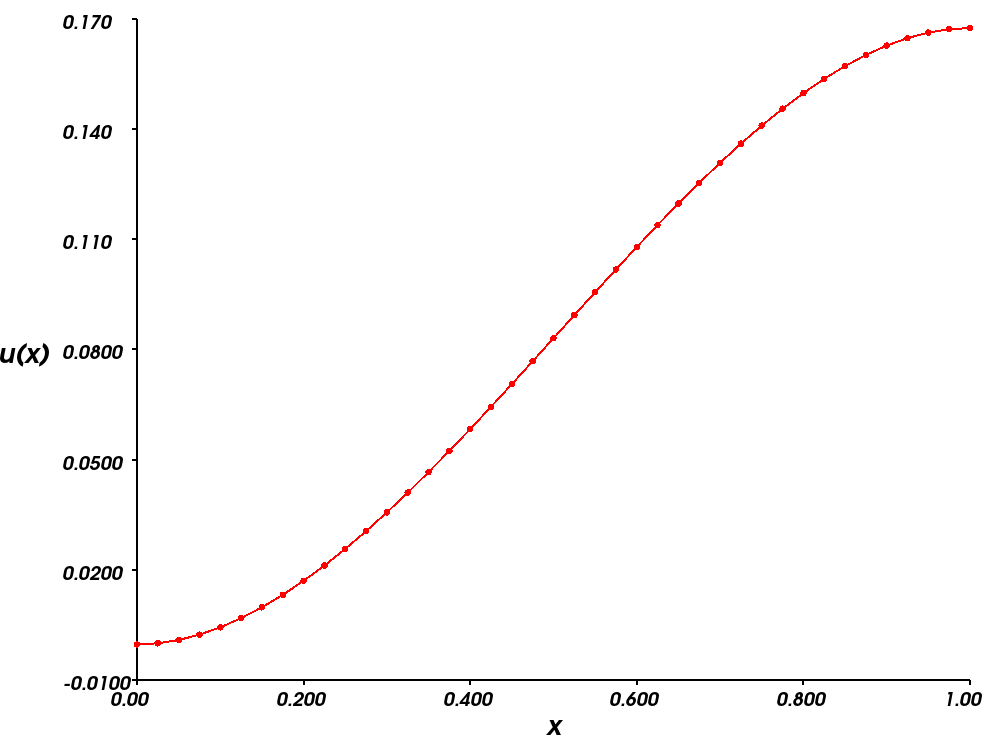
\includegraphics[scale=0.2]{images/ex_e_u.png}
\end{center}
\caption{The plot shows the numerical solution of eq. \eqref{eq:manufactured}}
\label{fig:ex_e_u}
\end{figure}

\begin{figure}[h]
\begin{center}
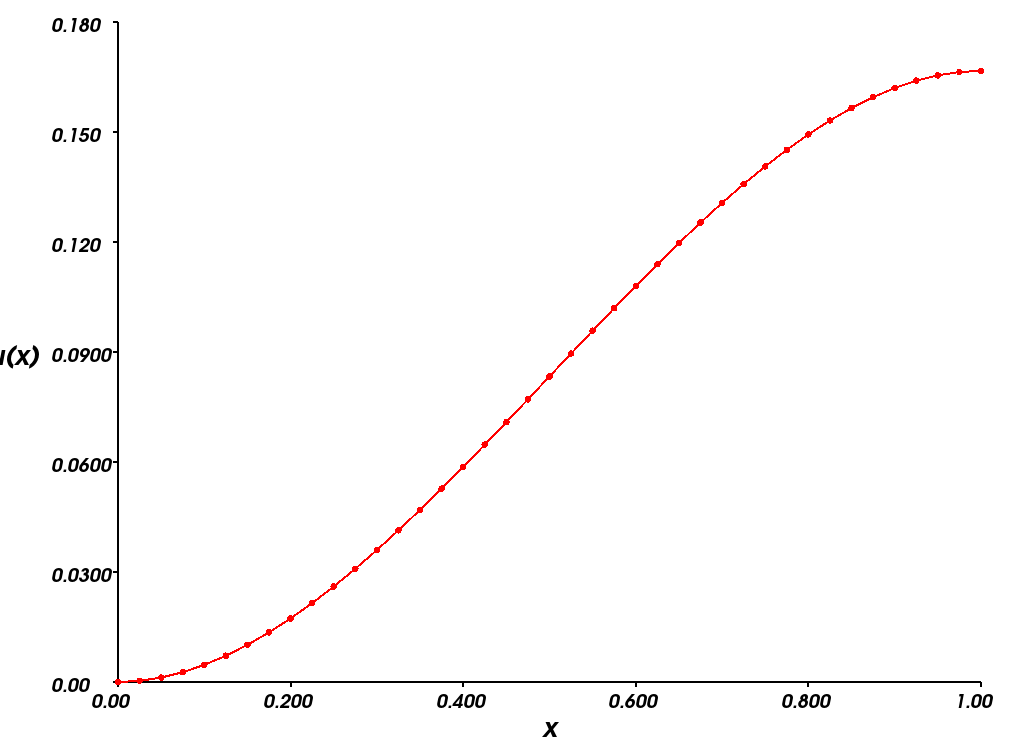
\includegraphics[scale=0.2]{images/ex_e_um.png}
\end{center}
\caption{The plot shows the exact solution of eq. \eqref{eq:manufactured}}
\label{fig:ex_e_um}
\end{figure}